\noindent

\includegraphics[height=1.25cm]{images/pictograms/replication}
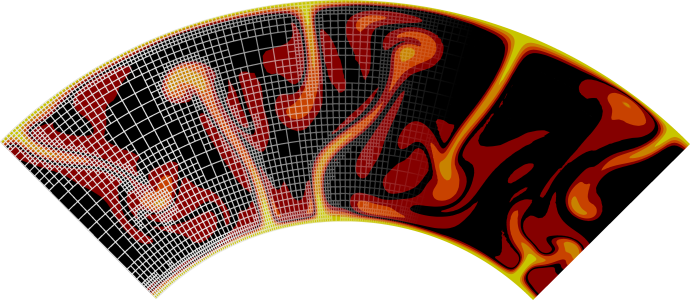
\includegraphics[height=1.25cm]{images/pictograms/aspect_logo}
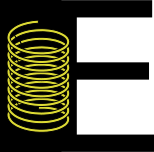
\includegraphics[height=1.25cm]{images/pictograms/elasticity}

\includegraphics[height=1.25cm]{images/pictograms/benchmark}

\includegraphics[height=1.25cm]{images/pictograms/under_construction}

\includegraphics[height=1.25cm]{images/pictograms/FEM}

\includegraphics[height=1.25cm]{images/pictograms/paraview}

\includegraphics[height=1.25cm]{images/pictograms/clean}

%%%%%%%%%%%%%%%%%%%%%%%%%%%%%%%%%%%%%%%%%%%%%%%%%%%%%%%%%%%%%%%%%%%%%%%%%%%%%%%%%%%%%%%%%%%%%%%%%%%

\begin{flushright} {\tiny {\color{gray} python\_codes/fieldstone\_186/text.tex}} \end{flushright}

%\lstinputlisting[language=bash,basicstyle=\small]{python_codes/template_keywords.key}

\par\noindent\rule{\textwidth}{0.4pt}

\begin{center}
\inpython
{\small Code: \url{https://github.com/cedrict/fieldstone/tree/master/python_codes/fieldstone_186}}
\end{center}

\par\noindent\rule{\textwidth}{0.4pt}

{\sl This stone was developed in collaboration with L. van der Wiel, A. Thompson}.

\par\noindent\rule{\textwidth}{0.4pt}

Last revision: October , 2026.

\par\noindent\rule{\textwidth}{0.4pt}

%%%%%%%%%%%%%%%%%%%%%%%%%%%%%%%%%%%%%%%%%%%%%%%%%%%%%%%%%%%%%%%%%%%%%%%%%%%%%%%%%%%%%%%%%%%%%%%%%%%

This \stone is based on:
\fullcite{vebo96}.

The paper gives an approximate analytic solution for a tunnel in a homogeneous elastic half
space, caused by ground loss and ovalization. The two basic processes are illustrated in
figure 1.

\begin{center}
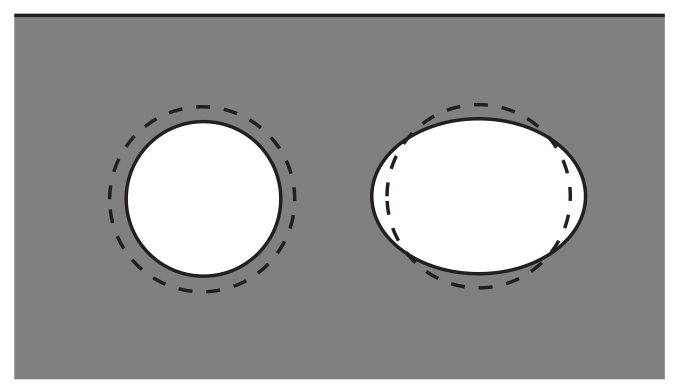
\includegraphics[width=8cm]{python_codes/fieldstone_186/images/fig1}\\
{\captionfont Ground loss and ovalization of a tunnel. Taken from \cite{vebo96}.}
\end{center}

The surface displacements for a tunnel in a semi-infinite medium are considered, as
well as the displacements and stresses throughout the elastic half space.
In what follows we disregard the ovalization, so $\delta=0$ (see paper).

Note that the pdf of the paper also contains additional material with 
full derivations of all fields. 


\newpage
%---------------------------------------
\subsection*{Analytical displacement}

\begin{center}
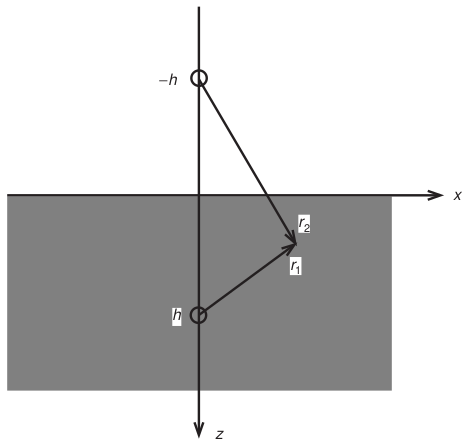
\includegraphics[width=4cm]{python_codes/fieldstone_186/images/fig2}
\end{center}

The total displacement is the sum of two components. The first is given by
Eqs 1,2 of \textcite{vebo96}:

\begin{eqnarray}
u_x &=& -\epsilon R^2 \left(  \frac{x}{r_1^2}+\frac{x}{r_2^2} \right) \nn\\
u_z &=& -\epsilon R^2 \left(  \frac{z_1}{r_1^2}+\frac{z_2}{r_2^2} \right) \nn
\end{eqnarray}

Also note that $u_z=0$ for $z=0$ since $z_1=-z_2$.
The second component is given by Eqs 10,11 of \textcite{vebo96}:

\begin{eqnarray}
u_x &=& -\frac{2\epsilon R^2 x}{m} \left( \frac{1}{r_2^2} - \frac{2mzz_2}{r_2^4}   \right) \nn\\
u_z &=&  \frac{2\epsilon R^2  }{m} \left( \frac{(m+1)z_2}{r_2^2} - \frac{mz(x^2-z_2^2)}{r_2^4}   \right) \nn
\end{eqnarray}
with $m=(1-2\nu)^{-1}$.

As stated in the paper, the complete solution is the sum of this solution and the previous 
expressions, i.e.:

\begin{eqnarray}
u_x &=& -\epsilon R^2 \left(  \frac{x}{r_1^2}+\frac{x}{r_2^2} \right) 
 -\frac{2\epsilon R^2 x}{m} \left( \frac{1}{r_2^2} - \frac{2mzz_2}{r_2^4}   \right) \nn\\
u_z &=& -\epsilon R^2 \left(  \frac{z_1}{r_1^2}+\frac{z_2}{r_2^2} \right) 
+  \frac{2\epsilon R^2  }{m} \left( \frac{(m+1)z_2}{r_2^2} - \frac{mz(x^2-z_2^2)}{r_2^4}   \right) \nn
\end{eqnarray}
Note that the factor $(m+1)/m$ in the equation above can also
be written as $2(1-\nu)$. 
Then velocity components can be written as follows:
\begin{eqnarray}
\frac{1}{\epsilon R^2} u_x 
&=& -  \left(  \frac{x}{r_1^2}+\frac{x}{r_2^2} \right) 
 - 2 \left( \frac{x (1-2\nu) }{r_2^2} - \frac{2xzz_2}{r_2^4}   \right) \nn\\
\frac{1}{\epsilon R^2} u_z 
&=& - \left(  \frac{z_1}{r_1^2}+\frac{z_2}{r_2^2} \right) 
+  2  \left( \frac{2(1-\nu)z_2}{r_2^2} - \frac{z(x^2-z_2^2)}{r_2^4}   \right) \nn
\end{eqnarray}


From the additional notes at the end of the paper we get\footnote{The 
'basic solution for ground loss' part of the additional notes 
needs to be discarded here. Also, these additional notes use the $y$
coordinate instead of $z$ in the paper so I have changed $y\rightarrow z$
because I will use the $y$ coordinate later.}:

\begin{eqnarray}
\frac{1}{\epsilon R^2} u_x &=&
-\left(\frac{x}{r_1^2}+\frac{x}{r_2^2} \right)
-2 \left(\frac{(1-2\nu)x}{r_2^2} - \frac{2xzz_2}{r_2^4} \right)
\nn\\
\frac{1}{\epsilon R^2} u_z &=&
-\left(\frac{z_1}{r_1^2}+\frac{z_2}{r_2^2} \right)
+2 \left(\frac{2(1-\nu)z_2}{r_2^2} - \frac{z(x^2-z_2^2)}{r_2^4} \right)
\end{eqnarray}
where $z_1=z-h$ and $z_2=z+h$, and which is identical to the expressions
of the original paper.

In particular the vertical component of the velocity at the surface is given by Eq 12:
\[
u_z(x,z=0)
= 2 \epsilon R^2 \frac{m+1}{m} \frac{h}{x^2+h^2}
= 4 \epsilon R^2 (1-\nu) \frac{h}{x^2+h^2}
\]

From Annie:
\begin{lstlisting}
def verruijt_displacement(x, epsilon=1/2000, R=1000, h=4000, nu=0.5):
    """Surface (z = 0) displacements from Verruijt & Booker (1996), delta = 0.
    epsilon > 0 means the cavity wall moves inward (ground loss).
    Returns (ux, uz) with ux positive in +x and uz positive DOWN.
        uz =  2*eps*R^2 * 2(1-nu) * h / (x^2 + h^2)
        ux = -2*eps*R^2 * 2(1-nu) * x / (x^2 + h^2)"""
    x = np.asarray(x, dtype=float)
    coef = 2.0 * epsilon * R**2 * 2.0 * (1.0 - nu)
    denom = x**2 + h**2
    return -coef * x / denom, coef * h / denom
\end{lstlisting}

Let us now formulate the equations above in Cartesian coordinates $x,y$, 
centered on the tunnel, with the $y$ axis pointing upwards.
In this case we have $z=L-y$, and then 
\begin{eqnarray}
z_1&=&z-h=L-y-L=-y  \\
z_2&=&z+h=L-y+L=-y+2L
\end{eqnarray}



\begin{center}
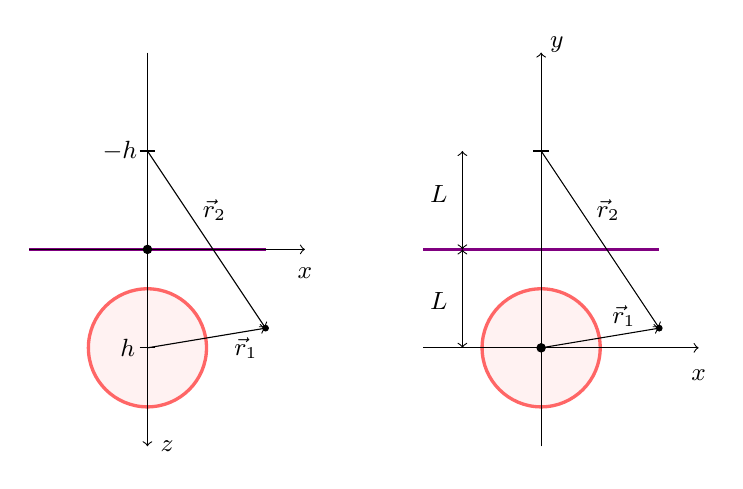
\begin{tikzpicture}
%\draw[fill=gray!23,gray!23](0,0) rectangle (10,7);
%\draw[step=0.5cm,gray,very thin] (0,0) grid (10,7); %background grid

\filldraw[color=red!60, fill=red!5, very thick]  (2,2.25) circle (0.75cm);
\filldraw[color=red!60, fill=red!5, very thick]  (7,2.25) circle (0.75cm);

\draw[very thick, violet] (0.5,3.5)--(3.5,3.5)  ; 
\draw[very thick, violet] (5.5,3.5)--(8.5,3.5)  ; 

%left
\draw[->] (0.5,3.5) -- (4,3.5)  ; 
\draw[->] (2,6) -- (2,1)  ; 
\node[] at (4,3.2) {\small $x$};
\node[] at (2.25,1) {\small $z$};
\draw[-] (1.9,2.25) -- (2.1,2.25)  ; 
\draw[-] (1.9,4.75) -- (2.1,4.75)  ; 
\node[] at (1.75,2.25) {\small $h$};
\node[] at (1.65,4.75) {\small $-h$};
\filldraw[black] (3.5,2.5) circle (1pt) ;
\draw[->] (2,2.25) -- (3.5,2.5)  ; 
\draw[->] (2,4.75) -- (3.5,2.5)  ; 
\filldraw[black] (2,3.5) circle (1.5pt) ;
\node[] at (3.25,2.25) {\small $\vec{r}_1$};
\node[] at (2.85,4) {\small $\vec{r}_2$};

%right
\draw[->] (7,1) -- (7,6)  ; 
\draw[->] (5.5,2.25) -- (9,2.25)  ; 
\node[] at (9,1.9) {\small $x$};
\node[] at (7.2,6.1) {\small $y$};
\draw[<->] (6,2.25) -- (6,3.5)  ; 
\node[] at (5.7,2.85) {\small $L$};
\draw[-] (6.9,4.75) -- (7.1,4.75)  ; 
\filldraw[black] (8.5,2.5) circle (1pt) ;
\draw[<->] (6,3.5) -- (6,4.75)  ; 
\node[] at (5.7,4.2) {\small $L$};
\draw[->] (7,2.25) -- (8.5,2.5)  ; 
\draw[->] (7,4.75) -- (8.5,2.5)  ; 
\filldraw[black] (7,2.25) circle (1.5pt) ;
\node[] at (8.05,2.65) {\small $\vec{r}_1$};
\node[] at (7.85,4) {\small $\vec{r}_2$};

\end{tikzpicture}
\end{center}

Likewise we have 

\begin{eqnarray}
r_1&=& \sqrt{(x-0)^2+(y-0)^2} = \sqrt{x^2+y^2}   \\
r_2&=& \sqrt{(x-0)^2+(y-2L)^2} = \sqrt{x^2+(y-2L)^2}
\end{eqnarray}


%---------------------------------------
\subsection*{Analytical stress}

In the original paper only the isotropic stress $\sigma_0=\frac12(\sigma_{xx}+\sigma_{yy})$
at the surface is presented in Eq 14 
\[
\sigma_0 = -4 \mu \epsilon R^2 \frac{z_2^2-x^2}{r_2^4}
\]

We need to turn to the additional material to find:

\begin{eqnarray}
\frac{1}{2\mu\epsilon R^2} \sigma_{xx}&=& 
\left( \frac{x^2-y_1^2}{r_1^4}+\frac{x^2-y_2^2}{r_2^4} \right) 
+2 \left( \frac{x^2-y_2^2}{r_2^4}-\frac{2yy_2(3x^2-y_2^2)}{r_2^6}  \right)
\nn\\
\frac{1}{2\mu\epsilon R^2} \sigma_{yy}&=& 
- \left(  \frac{x^2-y_1^2}{r_1^4}+\frac{x^2-y_2^2}{r_2^4}    \right) 
+2\left( \frac{x^2-y_2^2}{r_2^4}+\frac{2yy_2(3x^2-y_2^2)}{r_2^6}  \right)
\nn\\
\frac{1}{2\mu\epsilon R^2} \sigma_{xy} &=& 
 \left( \frac{2xy_1}{r_1^4}+\frac{2xy_2}{r_2^4}  \right)
+2 \frac{2xy(x^2-3y_2^2)}{r_2^6}
\nn
\end{eqnarray}


From Annie:
\begin{lstlisting}
def isotropic_stress_ver(x, z, R=1000, h=4000, epsilon=1/2000, mu=1e10):
    """Isotropic stress sigma_0 = (sigma_xx + sigma_zz)/2 from Verruijt & Booker
    (1996) Eq. (14) with delta = 0. Paper coordinates: z positive down, cavity
    centre at (0, h). Frame-independent, so valid in ASPECT's y-up frame."""
    x = np.asarray(x, dtype=float)
    z2 = np.asarray(z, dtype=float) + h
    r2s = x**2 + z2**2
    return -4 * mu * epsilon * R**2 * (z2**2 - x**2) / r2s**2
\end{lstlisting}

\newpage

Analytical solution in the tunnel walls:

\begin{center}
\includegraphics[width=5.7cm]{python_codes/fieldstone_186/RESULTS/circle_analytical_ux.pdf}
\includegraphics[width=5.7cm]{python_codes/fieldstone_186/RESULTS/circle_analytical_uy.pdf}
\includegraphics[width=5.7cm]{python_codes/fieldstone_186/RESULTS/circle_analytical_disp.pdf}\\
\includegraphics[width=5.7cm]{python_codes/fieldstone_186/RESULTS/circle_analytical_sigmaxx.pdf}
\includegraphics[width=5.7cm]{python_codes/fieldstone_186/RESULTS/circle_analytical_sigmaxy.pdf}
\includegraphics[width=5.7cm]{python_codes/fieldstone_186/RESULTS/circle_analytical_sigmayy.pdf}\\
\includegraphics[width=5.7cm]{python_codes/fieldstone_186/RESULTS/circle_analytical_sigma0.pdf}\\
{\captionfont All quantities have been normalised by $\epsilon R^2$.}
\end{center}

Analytical solution at the surface:

\begin{center}
\includegraphics[width=5.7cm]{python_codes/fieldstone_186/RESULTS/top_analytical_ux.pdf}
\includegraphics[width=5.7cm]{python_codes/fieldstone_186/RESULTS/top_analytical_uy.pdf}
\includegraphics[width=5.7cm]{python_codes/fieldstone_186/RESULTS/top_analytical_disp.pdf}\\
\includegraphics[width=5.7cm]{python_codes/fieldstone_186/RESULTS/top_analytical_sigmaxx.pdf}
\includegraphics[width=5.7cm]{python_codes/fieldstone_186/RESULTS/top_analytical_sigmaxy.pdf}
\includegraphics[width=5.7cm]{python_codes/fieldstone_186/RESULTS/top_analytical_sigmayy.pdf}\\
\includegraphics[width=5.7cm]{python_codes/fieldstone_186/RESULTS/top_analytical_sigma0.pdf}\\
{\captionfont All quantities have been normalised by $\epsilon R^2$.}
\end{center}








\begin{center}
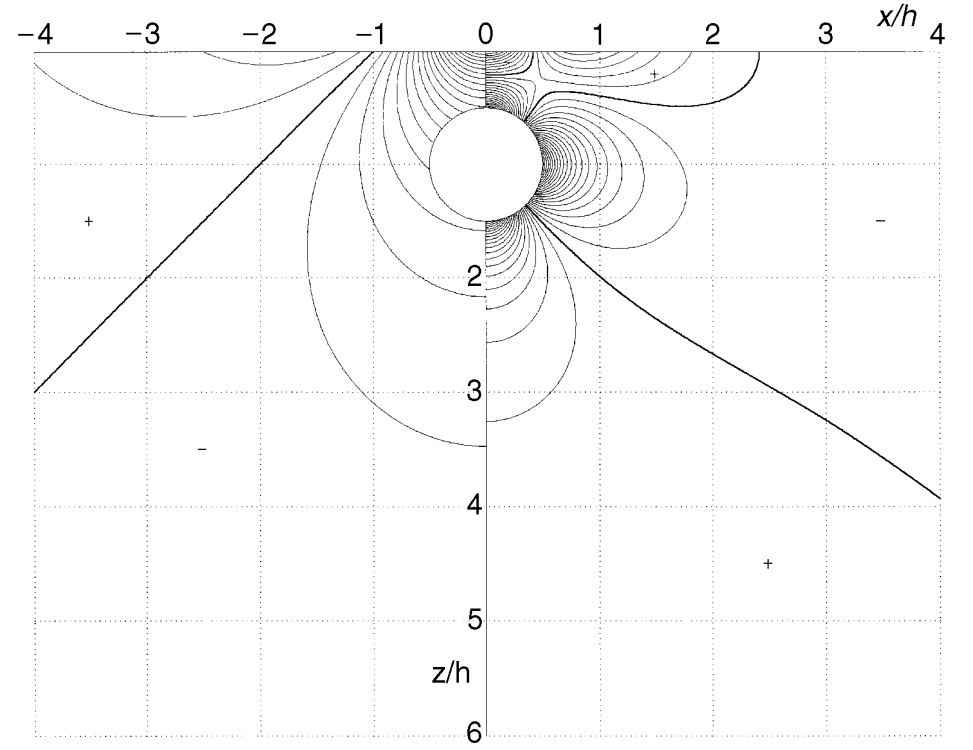
\includegraphics[width=8cm]{python_codes/fieldstone_186/images/fig4}\\
{\captionfont 
The left half of the figure shows
contours of $\sigma_0$ for the ground loss problem, and the
right half shows contours of $\sigma_0$ for the ovalization
problem. The thick lines indicate the contours for
$\sigma_0=0$, and the characters + and - indicate zones
of tension and compression respectively.  [...]
Although in Fig. 4 it has been assumed that $R/h=0.5$, the contours are 
valid for any value of $R/h$. It is interesting to note that in the case of
ground loss the stresses around the tunnel are all
compressive, whereas in the case of ovalization
there are zones of tension above and below the
tunnel. The construction of contours of other stress
components is a relatively simple and straight-
forward exercise.}
\end{center}



\newpage
%==========================
\section*{The GTECTON setup (experiment=1)}

The tunnel has a radius of 2~\si{\kilo\meter} and is situated 7~\si{\kilo\meter} below the surface.
The inside pressure is set to 5~\si{\mega\pascal}. The Poisson ratio is $\nu=0.35$ 
and the Young's modulus is $E=5\cdot 10^{10}~\si{\pascal}$.

This yields 
\[
\mu=\frac{E}{2(1+\nu)} = 
\]


\begin{center}
\includegraphics[width=8cm]{python_codes/fieldstone_186/RESULTS/GTECTON/VerruijtHorizontal.pdf}
\includegraphics[width=8cm]{python_codes/fieldstone_186/RESULTS/GTECTON/VerruijtVertical.pdf}
\end{center}


\newpage
%==========================
\section*{The ASPECT setup (experiment=2)}

The tunnel has a radius of 1~\si{\kilo\meter} and is situated 4~\si{\kilo\meter} below the surface.

Annie: 
``The tunnel displacement is the distance that the tunnel expands radially to create the perturbation. 
It's captured in the epsilon term in the paper.  Epsilon = tunnel displacement distance/ tunnel radius (R). 
You can see in my .vtu that velocity at the chamber border is 0.55m/yr, so I used 0.55m/1000m = epsilon.''

`` My isotropic stress function is straight from equation 14 and my displacement functions are 
equations 1 + 10 for x and 2 + 11 for z. And I simplified assuming that delta = 0 and z = 0. ''

``epsilon $>$ 0 means the cavity wall moves inward (ground loss)''

\begin{lstlisting}
nu=0.48
mu=1e10
E=2*mu*(1+nu)
lambdaa=E*nu/(1+nu)/(1-2*nu)
rad=1e3
Lx=4e3
Ly=4e3
\end{lstlisting}



\begin{center}
\includegraphics[width=8cm]{python_codes/fieldstone_186/RESULTS/ASPECT/ux.pdf}
\includegraphics[width=8cm]{python_codes/fieldstone_186/RESULTS/ASPECT/uy.pdf}
\end{center}





